% =====================================================================
% RAOD++ / iso-cost study — Results
% Every number is read from output/runs.csv and output/figdata/ .
% Figures are produced by scripts/make_figures.py from the same files.
% =====================================================================

\section{Results}
\label{sec:results}

\subsection{Enriching the training data does not help}
\label{sec:results:enrichment}

The control matrix of Section~\ref{sec:setup:enrichment} was run over ten seeds per
condition. Every treatment lands within $0.0025$ mAP$_{50\text{-}95}$ of the baseline, and
all of them fall \emph{below} it (Table~\ref{tab:enrichment}). Retrieval-based enrichment
exceeds the equal-budget control that adds no data by $0.0010$
(Holm-corrected $p = 0.0089$), a difference that is statistically detectable and, by the
criterion of Equation~\eqref{eq:floor}, practically negligible. The pre-registered success
criterion was not met against any of the three controls.

Two follow-ups rule out the obvious explanations. Training from scratch on the enriched
data rather than fine-tuning does not change the picture: the sign of the difference is not
even stable across seeds. Increasing the number of pasted instances per image, from $9{,}331$
to $22{,}874$ to $32{,}771$ per seed, leaves accuracy flat and then degrades it
($0.1862$, $0.1861$, $0.1786$ mAP$_{50\text{-}95}$; Figure~\ref{fig:budget-sweep}), so the
null result is not an artefact of too small an intervention.

\begin{figure}[t]\centering
  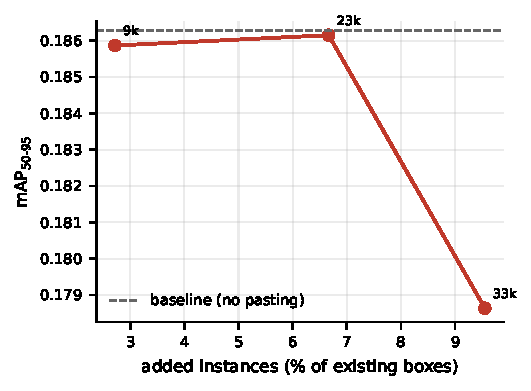
\includegraphics[width=0.62\linewidth]{fig/budget_sweep.pdf}
  \caption{Paste budget sweep on VisDrone, seed 42, trained from scratch: accuracy against
the number of added instances as a share of the $343{,}197$ existing training boxes. The
curve is flat to $6.7\%$ and falls at $9.5\%$, so the null result of
Table~\ref{tab:enrichment} is not explained by too small an intervention.}
  \label{fig:budget-sweep}
\end{figure}

\begin{table}[t]
\centering
\caption{Data-centric control matrix on VisDrone, ten seeds per condition. All conditions
start from the same checkpoint of the same seed and train for the same additional budget;
only the training data differs. Values from \texttt{output/F8\_v1\_primary.txt}.}
\label{tab:enrichment}
\begin{tabular}{llcc}
\toprule
Code & Condition & mAP$_{50}$ & mAP$_{50\text{-}95}$ \\
\midrule
E0 & baseline & $0.3310 \pm 0.0026$ & $0.1863 \pm 0.0015$ \\
E1 & equal budget, unchanged data & $0.3271 \pm 0.0027$ & $0.1839 \pm 0.0016$ \\
E2 & self-training pseudo-labels & $0.3267$ & $0.1838 \pm 0.0015$ \\
E3 & random-neighbour paste & $0.3276$ & $0.1845 \pm 0.0016$ \\
E4 & retrieval paste & $0.3276$ & $0.1845 \pm 0.0017$ \\
E5 & full pipeline & $0.3285 \pm 0.0029$ & $0.1849 \pm 0.0017$ \\
\bottomrule
\end{tabular}
\end{table}

\subsection{Retrieval carries information where the gallery is thin}
\label{sec:results:retrieval}

Although the enrichment does not improve detection, the retrieval stage itself is not
inert, and its behaviour is a finding in its own right. Measured over ten seeds,
consistency at $k = 5$ is $0.867$ micro-averaged and $0.618$ macro-averaged. Read per class
against the chance level of Equation~\eqref{eq:chance}, the pattern is monotone in the
gallery composition: for \emph{bicycle}, which occupies $0.3\%$ of the gallery, measured
consistency is $23.4$ times chance; for \emph{car}, at $58.9\%$, it is exactly chance
(Figure~\ref{fig:retrieval-consistency}). Retrieval carries the most information for the
classes the detector handles worst, and none at all for the class it already handles well.

\begin{figure}[t]\centering
  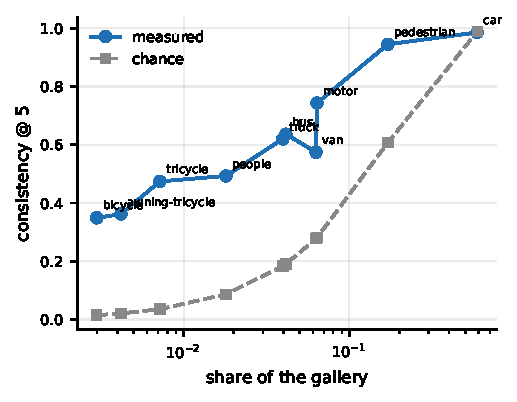
\includegraphics[width=0.62\linewidth]{fig/retrieval_consistency.pdf}
  \caption{Retrieval consistency at $k=5$ against the per-class chance level induced by gallery
composition, ten seeds. The ratio falls from $23.4\times$ for the rarest class to $1.0\times$
for the most frequent one.}\label{fig:retrieval-consistency}
\end{figure}
\begin{figure}[t]\centering
  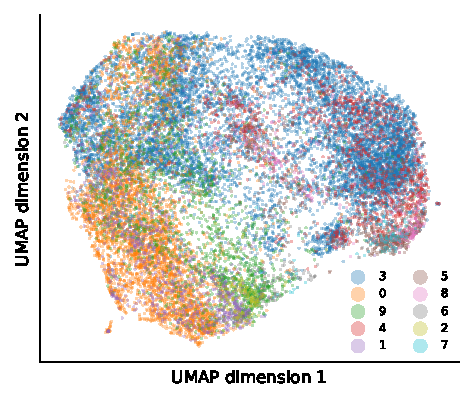
\includegraphics[width=0.55\linewidth]{fig/umap_lowconf.pdf}
  \caption{UMAP projection of the centred CLIP embeddings of low-confidence crops,
coloured by the class predicted by the detector. The frequent classes occupy broad
overlapping regions while the rare ones form small separated groups, which is the same
structure the consistency measurement reports numerically in
Figure~\ref{fig:retrieval-consistency}.}
  \label{fig:umap}
\end{figure}

\subsection{Confidence is honest, and that is the problem}
\label{sec:results:calibration}

A natural hypothesis for the failure above is that the detector is under-confident on small
objects, so that enrichment cannot help because the ranking, not the representation, is at
fault. Measured over ten seeds, the hypothesis does not hold. The gap between mean
confidence and empirical precision spans only $0.0295$ across size bands, and its sign runs
opposite to the hypothesis: the largest gap is on large objects ($-0.044$) and the smallest
on the tiniest ones ($-0.015$).

What the same measurement does show is the size of the operating-point problem
(Figure~\ref{fig:conf-precision}). At a deployment threshold of $0.5$, recall is $0.821$ for
large objects, $0.601$ for medium, $0.246$ for small and $0.053$ for the tiniest band.
Lowering the threshold to $0.1$ recovers only part of it, and at a precision cost: recall
for the tiniest band reaches $0.246$ with precision $0.278$. The detector's low confidence
on small objects is not miscalibration; it is an accurate report that the evidence is not
there.

\begin{figure}[t]\centering
  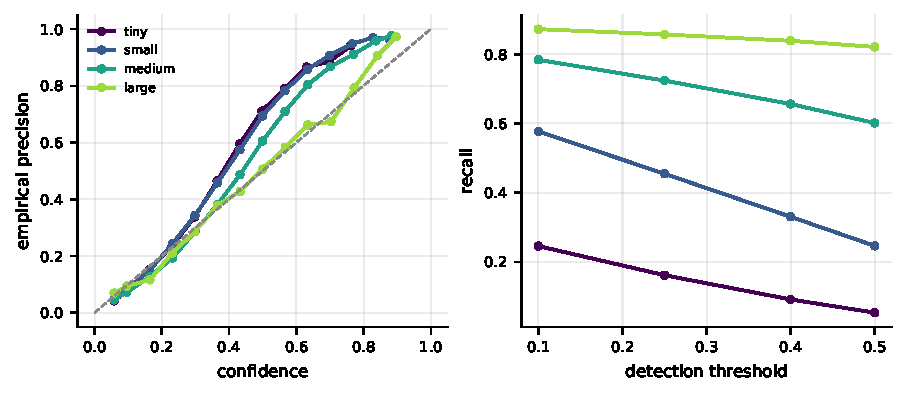
\includegraphics[width=0.98\linewidth]{fig/conf_precision.pdf}
  \caption{Left: empirical precision against confidence, by object size band. Right: recall at
deployment thresholds $\{0.10, 0.25, 0.40, 0.50\}$ per size band. Drawn from
\texttt{output/figdata/calib\_reliability.csv} and \texttt{calib\_operating\_point.csv}.}\label{fig:conf-precision}
\end{figure}
\subsection{Input resolution dominates the accuracy ladder}
\label{sec:results:resolution}

Table~\ref{tab:visdrone-grid} reports the full VisDrone grid with measured cost. Raising the
input from $640$ to $1536$ pixels lifts mAP$_{50\text{-}95}$ from $0.1863$ to $0.3249$, a
relative gain of $74\%$, against the $-0.0014$ obtained by the entire enrichment pipeline.
The per-step gains shrink but stay above the practical floor: $+0.0676$ from $640$ to $960$,
$+0.0446$ to $1280$, $+0.0264$ to $1536$. The curve has therefore not saturated at the
largest resolution tested (Figure~\ref{fig:resolution-curve}).

VisDrone frames are approximately $1360 \times 765$ pixels, so at $1536$ the network operates
on upsampled input and still improves. The gain cannot be attributed to additional image
information alone; the relative size of an object on the network's feature grid also
matters, since a $16 \times 16$ object spans roughly $2 \times 2$ cells at the P3 level with
$640$ input and about $5 \times 5$ at $1536$.

\begin{table}[t]
\centering
\caption{VisDrone grid, three seeds per condition, cost measured on an idle GPU as the
median of three batch-one passes. The baseline was additionally repeated over ten seeds.}
\label{tab:visdrone-grid}
\begin{tabular}{llccccc}
\toprule
Code & Model @ size & mAP$_{50}$ & mAP$_{50\text{-}95}$ & Latency (ms) & Power (W) & J/frame \\
\midrule
E0    & n@640      & $0.3310$ & $0.1863$ & $5.00$ & $58.3$  & $0.291$ \\
S640  & s@640      & $0.3884$ & $0.2239$ & $4.98$ & $94.7$  & $0.471$ \\
P640  & n-p2@640   & $0.3564$ & $0.2077$ & $5.51$ & $68.3$  & $0.376$ \\
R960  & n@960      & $0.4284$ & $0.2539$ & $5.50$ & $71.2$  & $0.392$ \\
S960  & s@960      & $0.4892$ & $0.2951$ & $5.61$ & $128.1$ & $0.719$ \\
P960  & n-p2@960   & $0.4426$ & $0.2667$ & $6.17$ & $95.8$  & $0.590$ \\
R1280 & n@1280     & $0.4899$ & $0.2985$ & $6.61$ & $85.9$  & $0.567$ \\
R1536 & n@1536     & $0.5245$ & $0.3249$ & $7.16$ & $109$   & $0.779$ \\
S1280 & s@1280     & $0.5423$ & $0.3360$ & $7.51$ & $143$   & $1.075$ \\
\bottomrule
\end{tabular}
\end{table}

\begin{figure}[t]\centering
  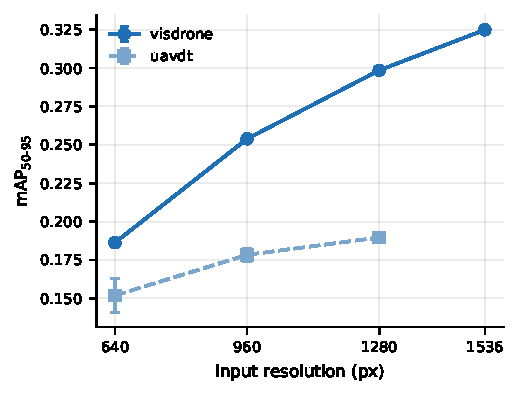
\includegraphics[width=0.62\linewidth]{fig/resolution_curve.pdf}
  \caption{Accuracy against input resolution for the nano model, three seeds, with measured latency
and energy annotated at each point. The curve has not saturated at $1536$.}\label{fig:resolution-curve}
\end{figure}
\begin{figure}[t]\centering
  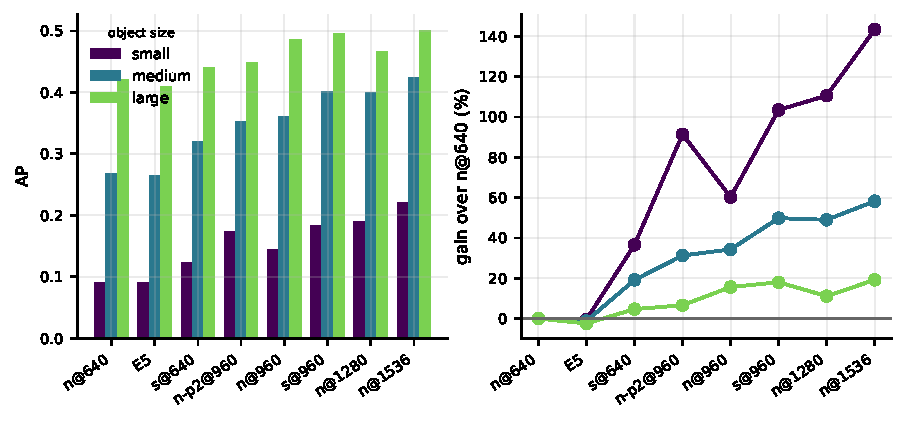
\includegraphics[width=0.98\linewidth]{fig/size_bands.pdf}
  \caption{AP by object size band (tiny / small / medium / large) for each condition, computed with
COCO-style evaluation. Drawn from \texttt{output/figdata/ap\_size\_bands.csv}.}\label{fig:size-bands}
\end{figure}
The gain is concentrated where the baseline is weakest. Between the $640$ baseline and
$1536$, AP on small objects rises from $0.0904$ to $0.2200$, a relative gain of $143\%$,
while AP on large objects moves from $0.4204$ to $0.5011$, a gain of $19\%$
(Figure~\ref{fig:size-bands}). The enrichment conditions, by contrast, leave every size
band unchanged: AP-small stays between $0.084$ and $0.090$ across all sixty runs.

\subsection{Which resource is scarce decides the answer}
\label{sec:results:isocost}

Accuracy alone favours capacity at the top of the ladder: S1280 reaches $0.3360$ against
R1536's $0.3249$. Accuracy alone is, however, the wrong comparison, because the two sit at
different cost. Applying the procedure of Section~\ref{sec:method:isocost} gives
Table~\ref{tab:isocost}.

On the latency axis the capacity arm leads by $0.0216$ mAP$_{50\text{-}95}$ over the
$5.02$--$7.01$\,ms range where both arms are measured. On the energy axis the ordering
reverses and the resolution arm leads by $0.0371$ over $0.474$--$0.765$\,J per frame. Both
differences clear the practical floor and survive Holm correction. The P2 head, the standard
architectural remedy for small objects in this literature, loses on both axes.

The mechanism is visible in the power measurements. Raising resolution moves board power
from $58.3$\,W at $640$ to $109$\,W at $1536$, while raising capacity moves it from
$94.7$\,W to $143$\,W at a lower resolution: reusing the same weights over more pixels costs
less power than moving more weights and activations. Latency at batch one does not reflect
this, because a model of this size does not saturate the device and a large share of the
wall-clock time sits in fixed overheads.

The gap also narrows as the budget grows, from $-0.0314$ at $5.02$\,ms to $-0.0101$ at
$7.01$\,ms on latency, and from $+0.0502$ at $0.474$\,J to $+0.0229$ at $0.765$\,J on
energy (Figures~\ref{fig:iso-latency} and~\ref{fig:iso-energy}). The allocation choice
matters most in the tight-budget regime, which is the regime an airborne platform operates
in.

\begin{table}[t]
\centering
\caption{Comparison at equal cost on VisDrone, three seeds, over the interval where both
arms have measurements. Positive values favour the resolution arm.}
\label{tab:isocost}
\begin{tabular}{llcccc}
\toprule
Axis & Comparison & Overlap & $\bar{\delta}$ & 95\% CI & $p_{\text{Holm}}$ \\
\midrule
Latency & resolution $-$ capacity & $5.020$--$7.013$\,ms & $-0.0216$ & $[-0.0219, -0.0210]$ & $0.0008$ \\
Energy  & resolution $-$ capacity & $0.474$--$0.765$\,J  & $+0.0371$ & $[+0.0360, +0.0378]$ & $0.0008$ \\
Latency & resolution $-$ P2 head  & $5.529$--$5.935$\,ms & $+0.0355$ & $[+0.0301, +0.0391]$ & $0.0059$ \\
Energy  & resolution $-$ P2 head  & $0.381$--$0.576$\,J  & $+0.0398$ & $[+0.0383, +0.0418]$ & $0.0014$ \\
\bottomrule
\end{tabular}
\end{table}

\begin{figure}[t]\centering
  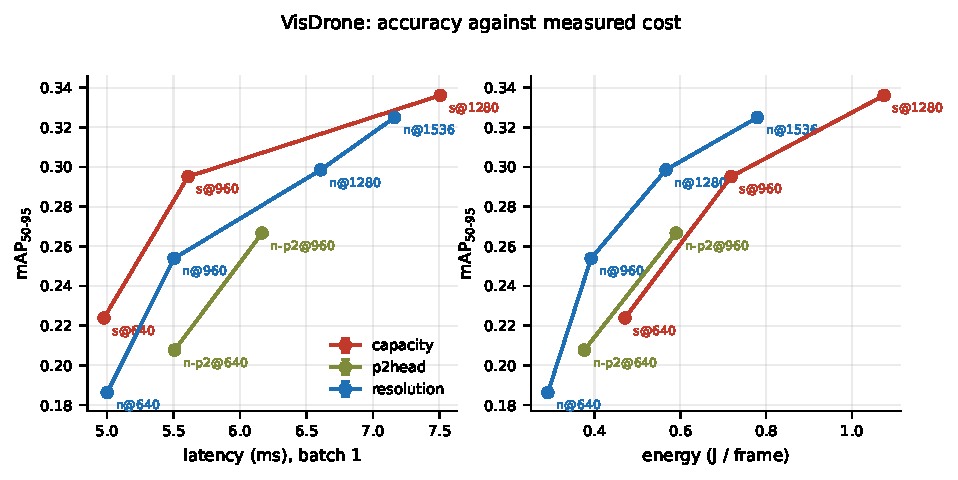
\includegraphics[width=0.98\linewidth]{fig/pareto.pdf}
  \caption{Accuracy against measured cost for every condition: latency on the left, energy per frame
on the right. Arms are drawn as connected curves; marker size encodes model capacity.}\label{fig:pareto}
\end{figure}
\begin{figure}[t]\centering
  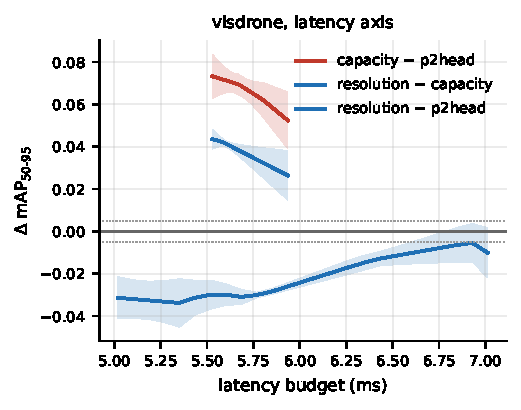
\includegraphics[width=0.62\linewidth]{fig/iso_latency.pdf}
  \caption{Difference between arms as a function of the latency budget, over the overlap interval
only, with the seed-wise spread shaded. Drawn from
\texttt{output/figdata/iso\_visdrone\_latency\_curve.csv}.}\label{fig:iso-latency}
\end{figure}
\begin{figure}[t]\centering
  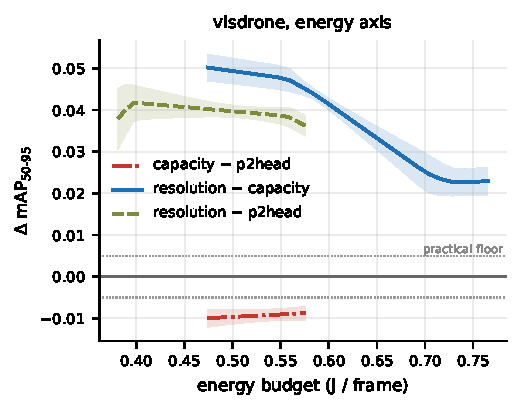
\includegraphics[width=0.62\linewidth]{fig/iso_energy.pdf}
  \caption{The same comparison on the energy axis. Drawn from
\texttt{output/figdata/iso\_visdrone\_energy\_curve.csv}.}\label{fig:iso-energy}
\end{figure}
\subsection{Transfer to a second dataset}
\label{sec:results:uavdt}

UAVDT tests whether the effect above is a property of UAV detection or of VisDrone's
particular scale statistics. Its objects are larger on average, so if the resolution
advantage is driven by small objects the effect should be weaker here. The official
sequence-level split is used, thinned to $4{,}840$ training and $1{,}854$ evaluation frames
with $84{,}727$ and $42{,}041$ boxes over three vehicle categories.

\textbf{H2 is not confirmed on UAVDT.} Both directions replicate --- capacity leads on latency,
resolution on energy --- with magnitudes of the same order as on VisDrone
($-0.0110$ and $+0.0148$ against $-0.0216$ and $+0.0371$), and both clear the practical
floor of Equation~\eqref{eq:floor}. What fails is statistical resolution: the corrected
$p$-values are $0.163$ and $0.085$ (Table~\ref{tab:uavdt-isocost}).

Two measured reasons. Seed variance is about seven times higher than on VisDrone, $0.0111$
against $0.0015$ mAP$_{50\text{-}95}$ for the $640$ baseline; training and evaluation come
from disjoint video sequences, and early stopping fires between $33$ and $83$ epochs rather
than $133$ to $178$. And the arms barely overlap: on the energy axis they share only
$0.444$--$0.506$\,J, a window of $0.062$\,J against $0.29$\,J on VisDrone, because here
they occupy largely separate regions --- resolution spans $0.20$--$0.52$\,J and capacity
$0.44$--$0.65$\,J.

That separation is itself informative: on UAVDT the resolution arm reaches accuracies in an
energy region the capacity arm cannot enter at all. Raising the seed count would narrow the
intervals but would not widen the overlap, and the analysis was not repeated with more
seeds after the outcome had been seen (protocol v2.4).

\begin{table}[t]
\centering
\caption{UAVDT grid, three seeds per condition, ordered by measured latency. Cost measured on an idle GPU as the median of three batch-one passes.}
\label{tab:uavdt-grid}
\begin{tabular}{llccccc}
\toprule
Code & Model @ size & mAP$_{50}$ & mAP$_{50\text{-}95}$ & Latency (ms) & Power (W) & J/frame \\
\midrule
R640  & n@640  & $0.2715 \pm 0.0143$ & $0.1518 \pm 0.0111$ & $4.56$ & $44.0$  & $0.201$ \\
S640  & s@640  & $0.2930 \pm 0.0156$ & $0.1678 \pm 0.0099$ & $4.74$ & $93.1$  & $0.442$ \\
R960  & n@960  & $0.3057 \pm 0.0129$ & $0.1783 \pm 0.0041$ & $5.14$ & $51.0$  & $0.262$ \\
S960  & s@960  & $0.3462$            & $0.2009$            & $5.27$ & $123.7$ & $0.652$ \\
R1280 & n@1280 & $0.3218$            & $0.1897$            & $6.82$ & $77.5$  & $0.524$ \\
\bottomrule
\end{tabular}
\end{table}

\begin{table}[t]
\centering
\caption{Comparison at equal cost on UAVDT. Holm corrects over $M=2$ comparisons, since the P2 arm was not run on this dataset. Positive values favour the resolution arm.}
\label{tab:uavdt-isocost}
\begin{tabular}{llcccc}
\toprule
Axis & Comparison & Overlap & $\bar{\delta}$ & 95\% CI & $p_{\text{Holm}}$ \\
\midrule
Latency & resolution $-$ capacity & $4.768$--$5.203$\,ms & $-0.0110$ & $[-0.0211, -0.0053]$ & $0.163$ \\
Energy  & resolution $-$ capacity & $0.444$--$0.506$\,J  & $+0.0148$ & $[+0.0089, +0.0196]$ & $0.085$ \\
\bottomrule
\end{tabular}
\end{table}

\begin{figure}[t]\centering
  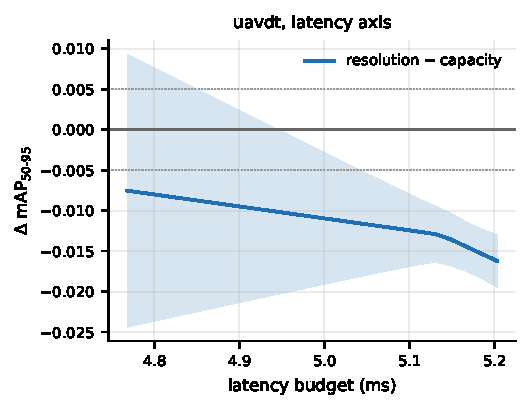
\includegraphics[width=0.49\linewidth]{fig/iso_uavdt_latency.pdf}
  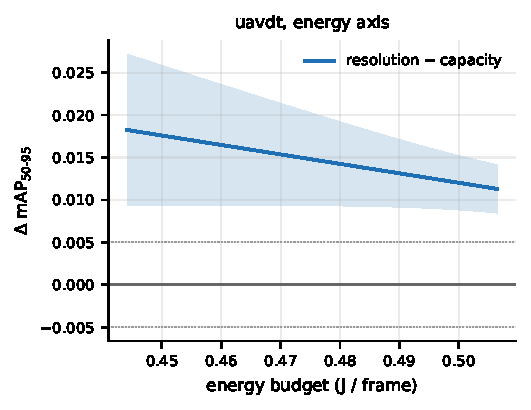
\includegraphics[width=0.49\linewidth]{fig/iso_uavdt_energy.pdf}
  \caption{Arm difference against budget on UAVDT, latency on the left and energy on the
right. Both directions match VisDrone (Figures~\ref{fig:iso-latency}
and~\ref{fig:iso-energy}); the shaded seed spread is far wider, which is why neither
reaches corrected significance.}\label{fig:iso-uavdt}
\end{figure}

\subsection{Convergence and qualitative behaviour}
\label{sec:results:qualitative}

Higher-resolution configurations do not merely end higher, they get there sooner. The
$1536$-pixel model passes the $640$ baseline's final accuracy at roughly epoch~$30$ of its
own schedule and continues to improve for the remainder
(Figure~\ref{fig:training-curves}). Early stopping fires at different points across
conditions, between $130$ and $200$ epochs on VisDrone, so the curves also show that no
condition was cut short relative to another.

Figure~\ref{fig:qualitative} shows what the size-band numbers look like on a frame. In a
scene annotated with $306$ objects, the baseline returns $161$ detections at a deployment
threshold of $0.25$ and leaves the dense cluster of distant vehicles and pedestrians almost
untouched; the capacity and resolution configurations return $201$ and $202$, and both
populate that region. The two recover a similar number of objects here, which is consistent
with the iso-cost analysis: they differ in what they cost, not in what they can see.

\begin{figure}[t]\centering
  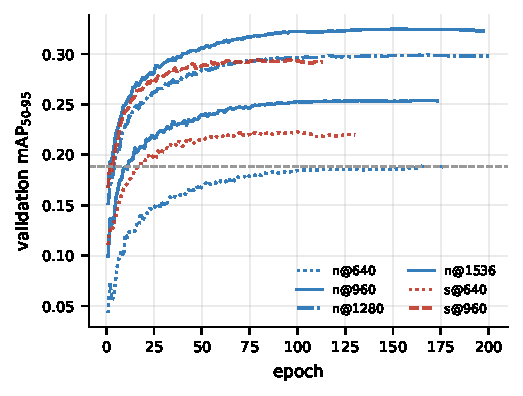
\includegraphics[width=0.62\linewidth]{fig/training_curves.pdf}
  \caption{Validation mAP$_{50\text{-}95}$ against epoch on VisDrone, averaged over seeds.
The dashed line marks the $640$ baseline's final accuracy. Drawn from
\texttt{output/figdata/training\_curves.csv}.}
  \label{fig:training-curves}
\end{figure}

\begin{figure*}[t]\centering
  \includegraphics[width=0.92\linewidth]{fig/qualitative.jpg}
  \caption{Detections at a deployment threshold of $0.25$ on the most densely annotated
validation frame. Top left: ground truth ($306$ boxes). Top right: baseline n@640
($161$ detections). Bottom left: capacity s@960 ($201$). Bottom right: resolution n@1536
($202$). Frames were selected by label count rather than by inspection, so the panel is
not a hand-picked success.}
  \label{fig:qualitative}
\end{figure*}
